\chapter{Algorithm and Model Creation}

\section{Execution Environment}

Execution occurs in a real-time partially synchronous environment.
Processes synchronize their clocks and execute steps of the election algorithm at predefined intervals.
Processes with clocks that are not sufficiently synchronized cannot form groups.
For this work, process execution occurs in an environment where the clocks are sufficiently synchronized to consistently form groups.

The execution environment is subject to omission failures.
In an omission failure, a message sent by one process to another process is lost in transit.
Omission failures can occur for many reasons.
Network congestion is a typical culprit.
Routers may drop packets or delay their delivery when there is a large amount of traffic or a network issue.
In a real-time environment, messages that are delayed and miss their real-time deadlines will have the same appearance as an omitted message.
Process delay can also cause a similar effect.
The execution environment for the election algorithm has a omission failure occurrence modeled as a Bernoulli trial.
In this model, each message has some probability $p$ of being delivered within the timing constraints imposed by the real-time schedule.
For the purpose of analyzing the effects of omission failures, processes are not subject to other faults.

\section{Election Algorithm}

A state machine for the election portion of the election algorithm is shown in Figure \ref{fig:statemachine}.
In the normal state, the election algorithm regularly searches for other coordinators to join with.
When another coordinator is identified, all other processes will yield to their future coordinator.
The method of selecting which process becomes the coordinator of the new group differentiates the invitation election algorithm from other approaches.
Regardless of the algorithm, the selection of the coordinator is always a race-condition and is difficult to model.

In the invitation election algorithm, processes are assigned a priority based on their process ID.
The coordinator with the highest priority is the first to send invites.
After a brief delay, if it appears that coordinator did not send their invites, the next highest process will send their invites.
Coordinators that receive invites will forward the invite to its group members.
Those processes will accept the invite.
Once a timeout expires, the coordinator will send a ``Ready'' message with a list of peers to all processes that accepted the invite.
The invited processes have timeouts for when they expect the ready message to arrive.
If the message does not arrive in time, the process will enter the recovery state where it resets to a group by itself.

\begin{figure*}[!t]
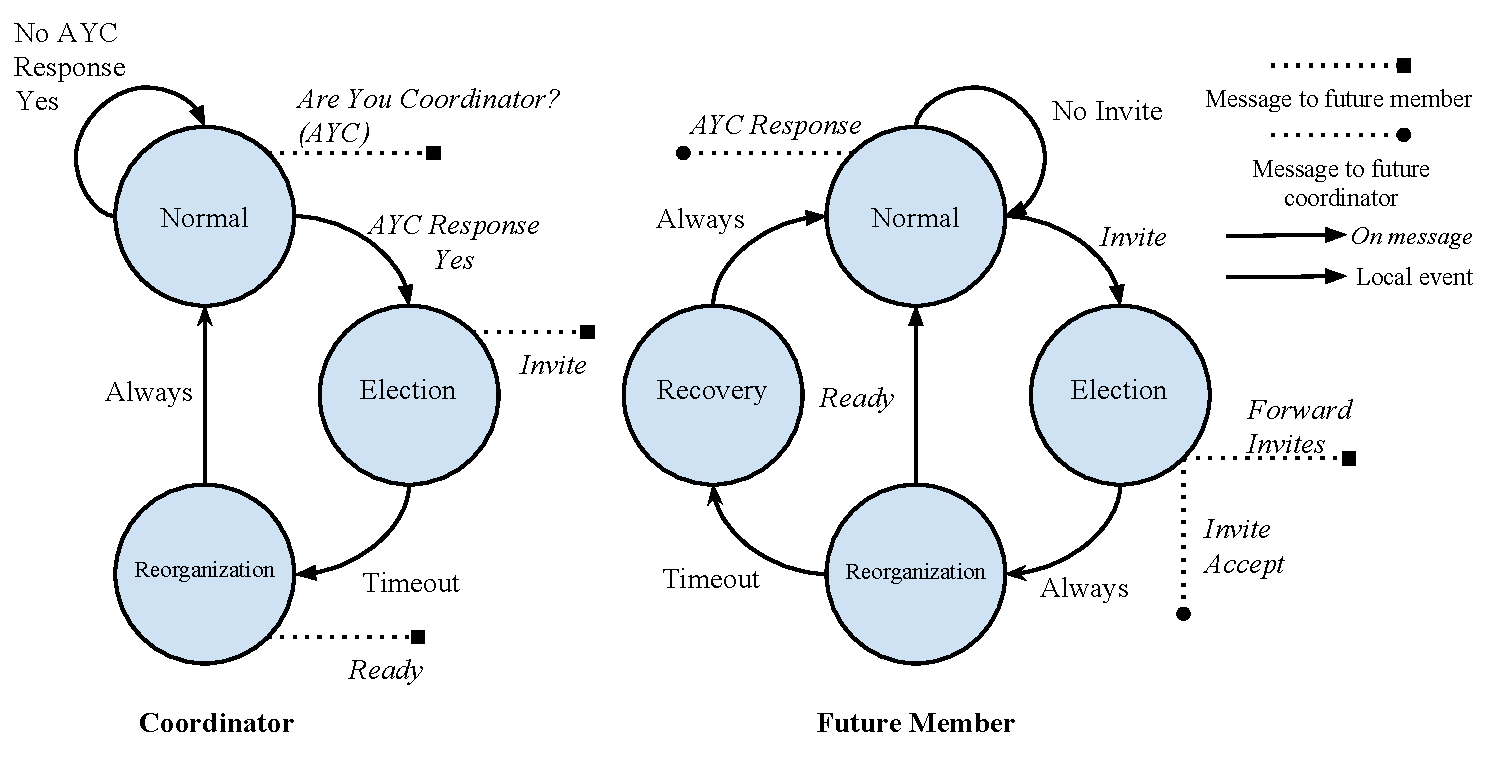
\includegraphics[width=\linewidth]{LeaderElectionStateDiagram.pdf}
\caption{State machine of a leader election. Processes start as coordinators in the ``Normal'' state and search for other coordinators to join with. Processes immediately respond to \ac{AYC} messages they receive. The algorithm was modified by adding a ``Ready Acknowledgment'' message as the final step of completing the election. Additionally, processes only accept invites if they have received an ``\ac{AYC} Response'' message from the inviting process.}
\label{fig:statemachine}
\end{figure*}

Once a group is formed it must be maintained.
To do this, processes occasionally exchange messages to verify the other is still reachable.
This interaction is shown in Figure \ref{fig:statemachine2}.
Coordinators send ``Are You Coordinator'' messages to members of its group to check if the process has left the group.
Group members send ``Are You There'' messages to the coordinator to verify they haven't been removed from the group, and to ensure the coordinator is still alive.
If processes fail to reply to received message before a timeout, they will leave the group.
Leaving the group can either be caused by the coordinator removing the process, or the process can enter a recovery state and leave the group, forming a new group by itself.

\begin{figure*}[!t]
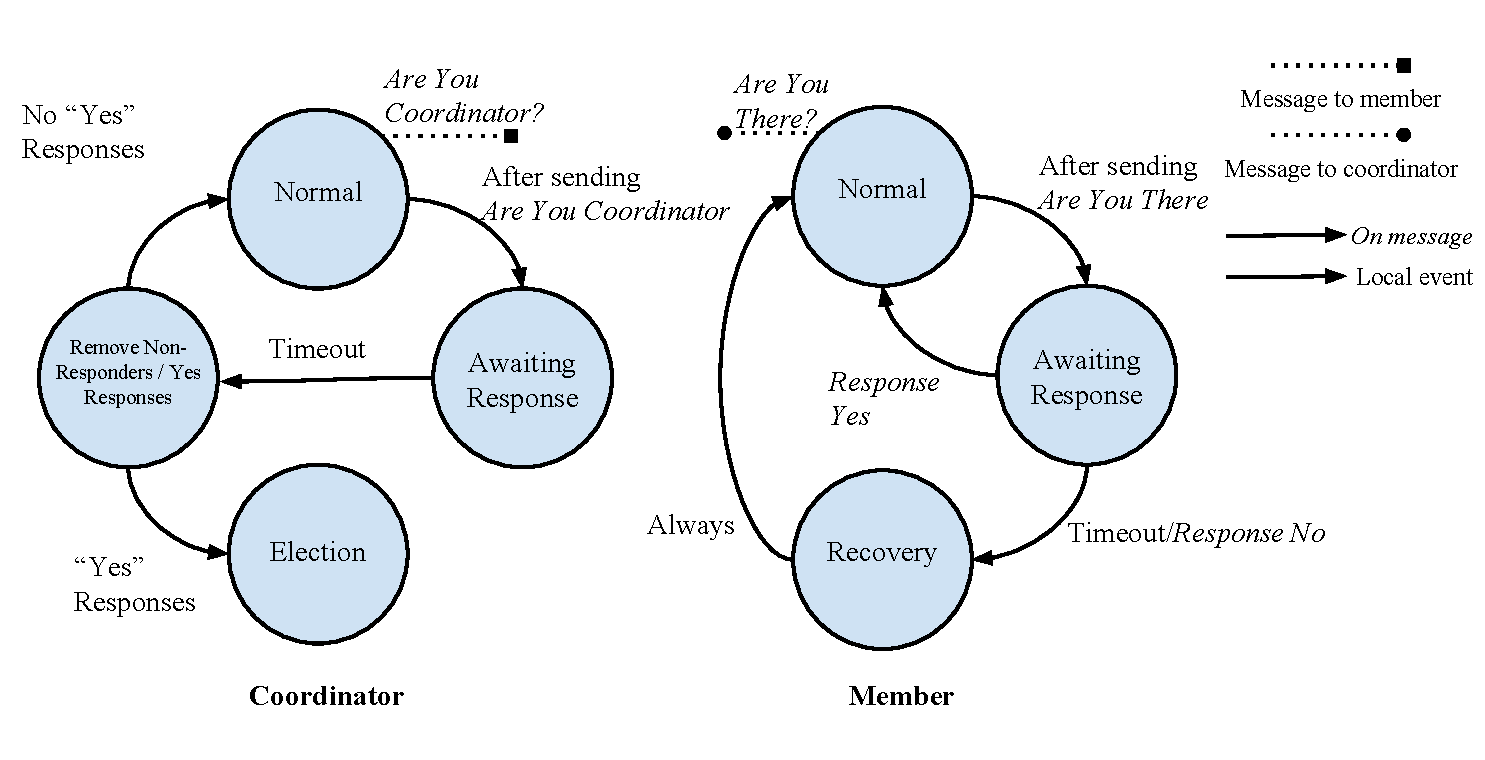
\includegraphics[width=\linewidth]{MaintainStateDiagram.pdf}
\caption{State machine of maintaining a group. The \ac{AYC} messages are the same as those in Figure \ref{fig:statemachine}. \ac{AYC} and \ac{AYT} are periodically sent by processes, and responses to those messages are immediately sent by the receiving process. In the modified algorithm, the member does not enter the recovery state if they do not receive an AYT response before the timeout expires.}
\label{fig:statemachine2}
\end{figure*}

For a variety of reasons modeling this algorithm is very difficult.
In a distributed system information cannot be instantaneously spread throughout the system.
As a consequence, an omission failure will cause a process to miss out on information distributed by other processes.
In particular, an omission of a ``Ready'' message sent to group members cannot be known to the coordinator without an additional message.
This missing information causes the coordinator's observation of the group to be out-of-date.
If the observed state of the group is incorrect, it cannot be used in a Markov chain with perfect information.
When the coordinator's observation of the group is out-of-date, a state observed by the coordinator would conflict with one observed by a member.
In this case, the state observed the member is closer to the true state of the system.
This situation is not favorable to modeling the formation of groups.
This is true because, for the purpose managing the group, the observations of the coordinator are much more valuable than those of the members.

In the modified algorithm, members have uncertainty with respect to their membership, and the coordinator has perfect information about members that definitely are a part of the group.
The original ``Are You There'' approach for detecting failure (Figure \ref{fig:statemachine2}) also causes a similar effect.
Additionally, the election algorithm has an inherent race condition as part of its normal operation.
This race condition can make the selection of the group leader inconsistent: the highest priority process may not always win the election.
For the purpose of analyzing the system, having a consistent leader is important for capturing a consistent view of grouping.
Additionally, the resulting leader of a normal election is difficult to model since it would necessitate capturing a race-condition in the model.

In this work, we modeled what a process will observe as a result of omission failure.
Therefore, it is important a process's observations hold to the Markov property.
The original Garcia-Molina algorithm has been modified so the observations of the coordinator process have the Markov property.
The following sections state the portions of the algorithm where the observation of the leader process does not yield the probability of next transition.
Changes to the algorithm relieved race conditions when selecting a leader, and made the state of the members a certainty for the coordinator.

Analysis is presented in the context of the \ac{FREEDM} \ac{DGI}. The \ac{FREEDM} \ac{DGI} is a portion of the \ac{FREEDM} project focusing on creating a distributed intelligence for controlling power electronics. As a consequence of managing the physical network of a critical infrastructure, the \ac{DGI} must execute in real-time: certain actions and tasks performed by the \ac{DGI} have to be completed in a specific time from.

To organize these agents, the system relies on existing clock synchronization techniques to put the system into a semi-synchronous execution environment. The \ac{DGI} is divided into several modules which focus on various tasks like autonomous configuration, managing power devices and collecting data from the system. \ac{DGI}s rely on synchronized clocks to begin the execution of the various tasks at the same time. This allows the message passing portions to specify deadlines to ensure that well-behaved participating agents are all working on similar tasks at the same time. For example, under the execution model as part of the autonomous configuration module, all agents begin the Leader Election Invitation Algorithm at the same time.

When reasoning about the system within the structure of the Markov Chains and MSDND security, this is a boon. An agent which is too out of sync will not be able to participate effectively and so is ignored for the purpose of this work. This effectively limits the state space of the complete naive model (as all agents are in roughly the same step of the algorithm). Furthermore, an agent can be sure that if message deliveries are timely (which is enforced by the real-time constraints) they can be certain of the lifetime of the inferred state.

This execution model has one major benefit: if, in order to participate in the algorithm, the agent must synchronize their actions (even if that synchronization is loose), the lifetime of a model is well established. In the case of a leader election algorithm, the agent that becomes the leader and constructs the model of the lifetime of the group can know for certain that another agent cannot come online and attempt to take over it's group until the next round of execution begins.

In the following portions of the paper we present an analysis of the information leakage for the original Garcia-Molina Invitation election algorithm and present how our modified version uses the MSDND information leakage to place certainty at one agent in order to construct a Markov model. In particular, we wish to use the MSDND model to show that the changes show that the coordinator can infer if each agent in the group considers itself a part of that agent's group.

Since any coordinated actions by a group must be initialized by the coordinator, having a model of the system constructed by the coordinator is the most valuable in the context of the system. The model constructed by this approach follows the $L$ state of the system. The $L$ state logically underestimates the state of the system, which is more accurate with respect to determining the current state for the next step of the algorithm. For the formulas presented, the coordinator of each group constructs a model of the system based on the cardinality of the the $L$ set based on the information flows in the algorithm.

\section{Group Maintenance and Leader Discovery}

The original and modified Garcia-Molina invitation election algorithms both use a common set of variables at each agent to track the state of the system.

Additionally, both versions use a recovery algorithm to abandon failed elections and groups.

Members cannot leave a group without the leader's permission.
Members do not suspect the coordinator has failed, only the coordinator may suspect the members.
This change is shown in Figure \ref{fig:statemachine2}, denoted by the elements marked with an asterisk.
For the purpose of starting an election, an \ac{AYT} message and its negative response are considered equivalent to a \ac{AYC} message and a positive response.
On receipt of the negative response, the member will immediately recover and become a leader.
This assumption relies on \ac{AYC} and \ac{AYT} messages being sent at roughly the same time.
This change leads to a live-lock situation in a crash failure, where the group's leader crashes and does not return and as a consequence the remaining members are trapped in a group without a leader.
For the purpose of this work, we have disregarded these live lock scenarios.

\subsection{Original Algorithm}

The \ac{AYC} message serves as a failure detector for crashed agents. In the models presented in this paper, crash failures are ignored as part of the modeled system.

The \ac{AYT} message serves as a check for the ``Ready'' message sent by the group leader at the end of the election algorithm. \ac{AYC} verifies the leader considers the sending process a part of its group.
A negative response to the \ac{AYT} message would prevent a process from participating in the current round of leader elections.
This violated the memorylessness property as a process would be excluded from the current round of elections based on an event that occurred the previous round.

\subsection{Modified Algorithm}

Algorithm \ref{alg:groupmnt} shows the modified components of the Invitation Election algorithm used for group maintenance and leader discovery.

\begin{algorithm}
\caption{Group Maintenance and Leader Discovery Functions}
    \label{alg:groupmnt}
\begin{algorithmic}[1]
\small
\Function{Check}{}
    \State This function is called at the start of a round by a leader
    \If {$State \neq Normal$ or $Coordinator \neq Me$}
        \Return
    \EndIf
    \State $Expected \gets \emptyset$
    \For {$j \in (AllPeers - \{Me\})$}
        \State $AreYouCoordinator(j)$
        \State $Expected \gets Expected \cup j$
    \EndFor
    \State Peers which respond ``Yes'' to $AreYouCoordinator$ are put into the $Coordinators$ set.
    \State Processes that respond are removed from $Expected$.
    \State When an $AreYouThere$ response is ``No'' and this process is a coordinator, the querying process is put in the $Coordinators$ set.
    \State Wait for responses, Peers that do not respond are removed from UpPeers.
    \State $UpPeers \gets (UpPeers-Expected) \cup {Me}$
    \State $UpPeers \gets (UpPeers-Coordinators) \cup {Me}$
    \If {$Responses = \emptyset$}
        \Return
    \EndIf
    \If {$Me < min(Responses)$}
        \State
        \Call{Merge}{Responses}
    \EndIf
\EndFunction

\Function{ReceiveAreYouThere}{Sender, Identifier}
    \If {$GroupID = Identifier$ and $Coordinator = Me$ and $Sender \in UpPeers$}
        \State Respond Yes
    \Else
        \State Respond No
        \State $Coordinators \gets Sender$
    \EndIf
\EndFunction
\end{algorithmic}
\end{algorithm}

In the maintenance portion of the algorithm, the leader acts on the set $L$, attempting to invite the agents not in its group into the group. Agents in $M$ but not $L$ will be re-invited. From the messages they receive from the leader the agents in $M-L$ will be able to infer that they are not a part of $L$. To accomplish this, the membership state of the process can be provided to the recipient as part of the \ac{AYC} message or it can be inferred from the process based on the response from an \ac{AYT} message. 

\begin{thm}
In a synchronous system a process in $M$ but not $L$ can determine its exclusion and act as though it was not in $M$, for the purpose of discovering leaders.
\end{thm}

An agent's membership in $M$ but not $L$ is secure to the agent in $M$ to the coordinator and from the coordinator to the agent. Let $\varphi_i$ indicate $j$'s membership in $i$'s group. The proof is identical to Theorem \ref{thm:captured}.

However, membership in $M$ is leaked by the next ``Are You There Message'' the agent sends.

\begin{table}[h!]
\centering
\small
\begin{tabularx}{\linewidth}{l X X}
1. & $I_{i,j} \varphi_{AYT}$ & $j$ sends an AYT message to $i$. \\
2. & $B_i I_{i,j} \varphi_{AYT} \wedge T_{i,j} \varphi_{AYT}$ & $i$ Trusts the message from j. \\
3. & $(j \not \in L \wedge j \in N \wedge \varphi_{AYT}) \rightarrow j \in M $ & Valuation membership. \\ 
\end{tabularx} \\~\\
$i$ knows $j$ is in $N_i$, but receiving the $AYT$ message leaks that $j$ considers itself part of $L_i$. Since $j$ is not a part of $L_i$, but considers itself to be, $j$ must be in $M$. Any message that implies $j$ belief in it's membership of $L_i$ is sufficient to include $j$ in $M$.
\end{table}`

Algorithms can potentially update $L_i$ based on information flow to include those agents in $M_i$.
However, in this instance, to ensure memorylessness, the process in $M_i$ must act in accordance with its exclusion from $L_i$.

\begin{thm}
A process in $M_i$ but not $L_i$ has the same likelihood of being in the next group as a process in not in $M_i$ and not in $L_i$.
\end{thm}

A process in neither $M_i$ nor $L_i$ must not have the \ac{AYC} message it sends and the response nor and have its own \ac{AYC} and that response omitted to reach the next step of the algorithm.
Successful completion depends on the delivery of 4 messages total.
If a process is in $M_i$ but not $L_i$, the same obligation follows, but that process sends and \ac{AYT} and expects that response, in addition to the \ac{AYC} from the coordinator.
Successful completion still depends on the delivery of 4 messages.

This approach allows the memorylessness property for the imaging to be upheld. If an agent is not in $L$ that agent will be able to determine it is not in $L$. This allows the same number of messages to be exchanged regardless of an agent's membership in $L$. If the probability that any given message sent to a process has a consistent probability of being delivered, the sequences of worlds that merge two coordinators has the same distribution of probable outcomes as the sequences of worlds that a process in $M$ but not $L$ is invited to the group.

\section{Coordinator Priority}

To alleviate the inherit race condition of leader selection, without loss of generality, a fixed leader process was selected.
This process was the only one that could become the leader of a multiprocess group.
This is shown in Figure \ref{fig:statemachine}, where only the selected process can send invite messages.
This simplification was applied because the configuration of the system with a larger number of processes depended on the configuration of the other processes.
Without this simplification, the state of the rest of the system would not have the memoryless property.
The state of the processes that are not in the observers group would change each round.
As a consequence the state of the rest of the system and the likelihood of forming a specific group size would change each step if other processes could become leader.
A probabilistic prediction would depend on how long the processes have been separated.
After a long enough period of time the distribution of states for the processes could be found using a steady-state analysis.
However, when processes enter the ``Recovery'' state they are deterministically placed in the alone state.
As a consequence the state of the system depends on the number of steps since the last reconfiguration, which violates the memoryless property.

Suppose P1 fails to detect P2 and P3 multiple times.
The probability P2 has grouped with P3 could then be modeled as a two process sub-case of this three process case.
Let this two process sub-case be described with a profile chain $P_{sub}$.
The probability of P2 and P3 joining P1's group depends on the state of the sub-case.
Additionally the probability distribution of an observation of the sub-case depends how many steps the sub-case has completed.
If $P_{sub}$ is ergodic, then $Steady(P_{sub}{}) \neq [1.0 \quad 0]$.
Each step of the sub-case ($n$) will move its distribution asymptotically closer to the steady-state:

\begin{equation} [1.0 \quad 0] * \lim_{n \to \infty}P_{sub}^n = Steady(P_{sub}) \end{equation}

Since the initial state of the algorithm in the sub-case must not be in a group ($[1.0 \quad 0]$), and the process is ergodic, the probability distribution of the sub-case depends on the number of steps ($n$).
As a consequence, the distribution for any $n$ must be different from the distribution of $n-1$.
Since the probability of P1 completing an election of P2 and P3 depends on the grouping of P2 and P3, the behavior of the full case cannot be memoryless, since it is a function of $n$.
Therefore, to make the algorithm memoryless, only a selected process may lead a multiprocess group.

Because elections can be triggered simultaneously, (and they always are in a synchronized execution model), a race condition exists in selecting the coordinator. In the original algorithm, the race condition was resolved using the agent identifier and a wait sequence. The agent that believed it had the lowest identification would immediately send invites, all other agents would wait some period of time before before sending theirs, in case the sender crashed. Our approach uses the maintenance and discovery phase to determine if an agent is the highest priority.

\subsection{Original Algorithm}

In the original algorithm, the break the race condition, each coordinator that has identified other coordinators to merge will determine if it should wait or immediately invite each agent it has identified as another coordinator. This action allows the agents to avoid sending all their invites at the same time.

The original text is vague on how this condition should be determined: if the coordinators should determine their wait time based on the global list of agents that could potential become leaders or if should be determined from the set of coordinators that that agent has identified as a fellow coordinator. In either case, the selection of when to send the invites influenced heavily by timing differences between the agents leading to non-deterministic behavior in many scenarios.

\subsection{Modified Algorithm}

\begin{thm}
With perfect information transfer, agents can determine the exact coordinator priority for each participating coordinator.
\end{thm}

If every agent has a unique identifier, then an algorithm that sends that identifier to each other process and receives and identifier from each other process, then that agent will know every identity in the network and will be able to determine it's priority relative to other participants.

\begin{thm}
Deterministic selection allows the likelihood of a particular invite being accepted to be computable for each agent.
\end{thm}

Querying an agent to see if they are a coordinator implies that the sending agent is a coordinator and implies that if that agent is not in a group with that agent and the querying agent is a coordinator, the receiving agent should expect to receive an invite from that agent, and will accept it if it is not already in a higher priority group, and it does not receive a message from a higher priority agent.

This approach of identifying priority during the group discovery phases allows the agents to determine when to send invites based on a deterministic measure rather than a probabilistic one based on execution ordering. A process can decide which invite it wishes to accept before the invites are sent out. There is a potential for live-lock in this approach if the highest priority process always crashes after other agents have determined they should accept that agents invite, but a similar scenario also exists in the original algorithm.

\section{Invitations}

\subsection{Original Algorithm}

In the original algorithm, a process accepts the first invitation it receives and does not accept any subsequent invitations.

\subsection{Modified Algorithm}

\begin{algorithm}
\caption{Invitation Functions}
\begin{algorithmic}[1]
\small
\Function{Merge}{Coordinators}
    \State This function invites all coordinators in Coordinators to join a group led by Me
    \State $State \gets Election$
    \State Stop work
    \State $Counter \gets Counter+1$
    \State $PendingID \gets (Me,Counter)$
    \State $Coordinator \gets Me$
    \State $Pending \gets UpPeers - {Me}$
    \For {$j \in Coordinators$}
        \Call{Invite}{j,Coordinator,PendingID}
    \EndFor
    \State Wait for responses, Peers that accept the invite are added to $Pending$.
    \State $State \gets Reorganization$
	\State $GroupID \gets PendingID$
	\State $UpPeers \gets Pending$
    \For {$j \in UpPeers$}
        \Call{Ready}{j,Coordinator,GroupID,UpPeers}
    \EndFor
    \State $Expected \gets UpPeers$
    \State Wait for responses, Peers that acknowledge are removed from $Expected$
    \State $UpPeers \gets UpPeers - Expected$
    \State $State \gets Normal$
\EndFunction

\State

\Function{ReceiveInvitation}{Sender,Leader,Identifier}
    \If {$State \neq Normal$}
        \Return
    \EndIf
    \If {$Sender < Coordinator$}
        \Return
    \EndIf
    \State Stop Work
    \State $PendingID \gets Identifier$
    \State $State \gets Election$
    \State $Accept(Coordinator,Identifier)$
    \State $State \gets Reorganization$
    \If {$Ready$ is not received}
        \State $Recovery()$
    \EndIf
\EndFunction

\State

\Function{ReceiveAccept}{Sender,Leader,Identifier}
    \If {$State \gets Election$ and $PendingID = Identifier$}
        \State $Pending \gets Pending \cup {Sender}$
    \EndIf
\EndFunction

\Function{ReceiveReadyAcknowledge}{Sender}
    \State $Pending \gets Pending \cup {Sender}$
\EndFunction

\end{algorithmic}
\end{algorithm}

In the invitation portion of the algorithm, the sender of the invite is confident the agent has accepted the invite because the accept message arrives. The group list that the new leader prepares for the ready message is an $N$ set of the potential group members. The list is distributed to the new members. Agents that do not receive $N$ or fail to send a receipt message are not in $L$. Algorithms that depend on the set of agents in the group will act on $N$. There is a potential that to the leader the agents in $N$ but not $L$ will act as though they are part of the group. Algorithmically, the leader can then expand $L$ to cover the information leaked by that agent acting as though it is holds a state that makes it part of $L$.

An agent can determine the likelihood that its group will form in a particular configuration if it is the highest priority agent. The determination of coordinator priority is determined during the check phase, then an agent can determine if it is the highest priority agent. If an agent determines it is the highest priority, it can then easily determine the probability that any given agent receives it's invite message and that the response to that invite message returns to that agent.

An agent can determine the likelihood that its group will form a particular configuration if it can determine the likelihood that agents with higher priority do not form a group with with the agents in that configuration.

If the determination of the coordinator priority reveals that an agent has a lower priority than 1 other agent, the probability that an agent accepts and invite from the agent is the probability the other agent does not recognize the other agent's priority (which is based on the delivery of the check messages).

Alternatively, if the determination of the coordinator priority reveals that an agent has a lower priority than $n$ ($n > 2$) other agents, the probability that some other agent will accept that agents invite is the probability that for each of the other agents ($n-1 ... 0$) the invited agent does not recognize that agent's priority.

\section{Ready State}

The changes added a third message to completing an election -- a ``Ready ACK'' message, shown in Figure \ref{fig:statemachine}.
This message is sent by a member after receiving the ready message from the coordinator.
This message induces a causality that allows the coordinator to be certain of the member's status before the next round.
Without the ready acknowledgment, the member may not receive the ready message and the coordinator will observe the member is a part of the group.
This interaction is shown in Figure \ref{fig:lostready}.

\begin{figure}
\begin{centering}
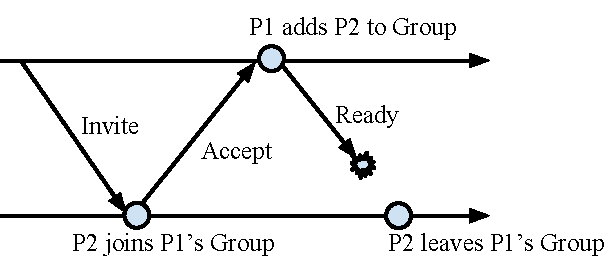
\includegraphics[width=0.6\linewidth]{LostReady.pdf}
\caption{The grouping processes effects the outcome of elections} \label{fig:lostready}
\end{centering}
\end{figure}

Without the ready acknowledgment message, the probability a member remains in a group in the first round after an election has a different probability than each subsequent round.
By adding the extra message, the observation of the coordinator must be the state of the member of the group.
As a consequence, the probability a member remains in a group in the first round after an election is identical to each subsequent round.

\subsection{Original Algorithm}

In the original algorithm the list of agents in the group is distributed as part of the ready message. Based on analysis presented earlier in the paper, since there is no confirmation of receipt for the ready message, the leader cannot determine the actual state of the group has it only has the set of wffs with no valuation function describing the group state $N_i$.

\subsection{Modified Algorithm}

\begin{thm}
Ready and Ready Acknowledge result in the leader holding and $L$ state and the members holding a $N$ state.
\end{thm}

Proof: This result is based partially on the non-deducibility results presented previously in the Two-Armies problem. Let $I_{i,j} \psi_j$ be an agent $j$ sending an invite accept to agent $i$.

\begin{table}[h!]
\centering
\small
\begin{tabularx}{\linewidth}{l X X}
1. & $I_{i,j} \psi_k \forall j $ & Each agent $j$ that accepts the invite does so.  \\
2. & $I_{j,i} \{ \varphi_k \forall k \}$ & $i$ sends $\varphi_i$ to $j$ (Ready Message). \\
3.a. & $w \not \vDash V_{B_j \varphi_k}^i(w) $ & $i$ has no means of determining if $j$ received the ready message. \\
3.b. & $B_{j}I_{j,i} \varphi_k \wedge T_{j,i} \varphi_k \forall \varphi_k$ & $j$ Trusts the contents of the Ready message. \\
4.b & $B_j B_i \varphi_k \forall \varphi_k$ & By C1. \\
5. & $w \vDash V_{B_i \varphi_k}^j(w)$ & $j$ believes that $i$ believes $k$ is part of the group. \\
6. & $I_{i,j} \gamma_j \wedge B_i I_{i,j} \gamma_j \wedge T_{i,j} \gamma_j$ & $i$ receives the Ready Acknowledge. \\
7. & $B_i \gamma_j \rightarrow w \vDash V_{B_j \varphi_k}^{i}(w) \wedge B_i \varphi_j$ & $i$ knows that $j$ believes the $N_i$ set and knows that $j$ is a part of the $L_i$ set. \\
\end{tabularx} \\~\\
The proof repeats for each $j$ that successfully delivers an invite accept message to $i$. Therefore, $j$ has the $N_i$ set and $i$ has the $L_i$ set.
\label{tab:readylnsetproof}
\end{table}

In the modified algorithm, the agents that receive the ready message reply with confirmation. This allows the leader of the group to determine $L_i$, a set of agents that have definitely received the ready message. By coupling this with the other modifications to the algorithm, for the semi-synchronous execution environment used by the \ac{DGI}, the states observed by the leader are memoryless.

\section{Composed Algorithm}

In the specified execution environment, each time before the coordinator runs the check portion of the election algorithm it produces an image of the current world to use as the first state of the constructed Markov chain. Each agent in the system has the stability property. As part of the stability property any wffs whose information was transferred after the last image was taken cannot change until the process takes the newest image. For the election algorithm, this causes the leader to doubt the values in $L$.

If a process is not in $L$ it will have to go through the election procedure even though it may be in $M$. This ensures that the sequence of changes necessary to bring that agent into the group is identical whether regardless of the agent's membership in $M$, ensuring the memorylessness property. Previous work \cite{JOURNAL} describes this algorithm and shows a Markov chain accurately describing the behavior of an implementation of this algorithm.

\subsubsection{Creation of A Profile Chain}

The election algorithm produces and distributes a set of processes $UpPeers$ and a coordinator of that set.
$UpPeers$ is distributed via message passing and maintained by the coordinator.
Different processes may have different versions of $UpPeers$ for a given coordinator as processes enter and leave the group.
However, a process will eventually receive an up-to-date version of $UpPeers$ from the coordinator, or it will leave the group.

To model the behavior of the algorithm, at each time-step the selected process recorded the cardinality of its membership set $UpPeers$.
The selected process was always the coordinator of any formed group, and was the only process that could lead a multi-process group.
The cardinality of $UpPeers$ directly mapped to the state in the Markov Chain.
For example given the membership set $S=\{P1,P2,P3\}$, then $\left | S \right |=3$ and the state of the system in the Markov chain is also $i=3$.

The profile Markov chain for the algorithm was constructed as a closed form representation of the algorithm's behavior.
In each round, the behavior is described by two components: maintaining a group and inviting other processes into the group.
The coordinator will exchange an ``Are You Coordinator'' message and the peer will respond to verify is still available.
To maintain a group of $m$ other processes, the probability is defined as a random variable with the following \ac{pdf}:

\begin{equation}
 \Pr_{M}(X=k; m) =
   \begin{cases}
    \binom{m}{k} p^{2k}(1-p^2)^{m-k}, & \text{if } 0 \leq k \leq m \\
    0,                                & \text{otherwise} \\
  \end{cases}
\end{equation}

Where $k$ is the number of processes remaining in a group selected from $m$ processes.
A process will leave a group if, from the considered process's perspective, they do not respond to an ``Are You Coordinator'' message.
Members cannot change their state without coordinating with the leader.

To invite other processes to the group, the two processes ultimately exchange up to 8 messages.
In a round, a single process can invite many other processes to its group.
From a selection of $n$ other coordinators, the probability distribution for joining a new group with $k$ of the $n$ processes is:

\begin{equation}
	\Pr_{I}(Y=k; n) =
	\begin{cases}
		\binom{n}{k} p^{8k}(1-p^8)^{n-k}, & \text{if } 0 \leq k \leq n \\
		0,                                & \text{otherwise} \\
	\end{cases}
\end{equation}

In the profile chain, in a state $s$ that describes the number of processes in a group, the probability of transitioning from $s$ to $s'$ with $n$ total processes (including the considered process) is:

\begin{align} \Pr_{T}(Z=s'; n; s) = \sum_{i=0}^{s-1} &\Pr_{M}(X=i; s-1) \cdot
\nonumber \\ &\Pr_{I}(X=s'-i; n-s-1) \end{align}

From this distribution, a set of transition probabilities can be calculated for a given omission rate $p$ and number of processes $n$.
This set of transition probabilities forms a profile Markov chain $P$, which can be evaluated to for any number of processes $n$ and omission rate $p$.
The generated profile chain is ergodic when $0<p<1.0$. The profile chain is a stationary Markov chain.

\section{Model Validation}

%State that verification of the profile chain via statistical tests is important. State that if P and T are ergodic stochastic sources and can generate similar sequences if they have the same transition probabilities. State that statistical tests can identify if two chains are different at some significant level.

To assert the closed form profile chain accurately represents the implementation of the algorithm, it must be validated.
Since $T$ and $P$ are ergodic, they can be checked for equivalence using a goodness-of-fit test.
If the goodness-of-fit test indicates the chains are equivalent, they will generate similar sequences and have similar properties when analyzed.
Therefore, generated $P$ chains can be used to analyze the behavior of the algorithm during live execution with changing conditions.

To verify the test chain $T$ is equivalent to the profile chain $P$, a $\chi^2$ goodness-of-fit test is employed.
The null-hypothesis of this test ($H_{0}$) asserts the profile chain $P$ is equivalent to the test chain $T$:

\begin{equation} H_{0}: T = P \end{equation}

With an alternative hypothesis that the two chains are not equivalent:

\begin{equation} H_{1}: T \neq P \end{equation}

The $\chi^2$ test measures the goodness-of-fit for a complete chain by combining the measurements of goodness of fit for the transitions away from each state.
Therefore, the goodness of fit test for the chain is a summation of tests for each state:\cite{MARKOV3}

\begin{equation} \chi^2 = \sum_{i}^{m} \sum_{j}^{m} = \frac{n_{i}(P_{ij}-T_{ij})^2}{P_{ij}} \end{equation}

Where $n_{i}$ is the number of times the state $i$ was observed in the input sequence used to construct the test chain $T$.
The summation is distributed as $\chi^2$ with $m(m-1)$ \ac{DF} if all entries in $P_{ij}$ are non-zero.
In this work, all transitions in the profile Markov chain $P$ are non-zero when $0<p<1.0$.
However, the probability of some transitions may be extremely small.
The $\chi^2$ value was compared to a \ac{CV} giving a measure of how likely it was $H_{0}$ could not be rejected.
This work selected an $\alpha = 0.05$ significance level to reject the hypothesis $T=P$.

If the hypothesis $H_{0}$ were to be rejected, it would indicate the test chain and profile chain differ significantly.
As a consequence of rejecting the hypothesis, the implementation would have behavior from the generated closed form solution.

To verify the model, it was compared to runs of an implementation of the algorithm.
Test data was collected for systems with 3, 4, 5 and 6 processes.
Information was collected from sufficiently long runs of the system with an omission rates between 0.05 and 0.95 tested at intervals of 0.05.
Table \ref{tab:chisummary} shows the measured error and p-value for the worst observed error for each number of processes.
Since the measured error is less than the critical value and the p-value is greater than 0.05, we cannot reject $H_0$. 
As a consequence, the profile chains ($P$) are representative of the behavior of the algorithm's implementation.

\begin{table*}[!t]
\centering
\begin{tabular}{ c | c c c c c}
  \hline
  Processes & DF & CV & Worst Error & $\Pr(WorstError)$ &  p-value \\ \hline
  3 & 6 & 12.6 & 8.90 & 0.80 & 0.18 \\
  4 & 12 & 21.0 & 14.55 & 0.75 & 0.27 \\
  5 & 20 & 31.4 & 23.47 & 0.65 & 0.27 \\
  6 & 30 & 43.8 & 32.69 & 0.85 & 0.34 \\
\end{tabular}
\caption{Summary of $\chi^2$ tests performed.}
\label{tab:chisummary}
\end{table*}

\section{Profile Chain Analysis}

Resources can only be managed effectively when multiple \ac{DGI} coordinate together to manage those resources.
Without another DGI to coordinate with, the DGI has a limited range of options to manage power generation, storage and loads.
Therefore, the amount of time DGI will spend coordinating with another process is of particular interest.
\cite{CRITIS2012} defines an \ac{IGT} metric to measure the amount of time a DGI process spends coordinating with at least one other process.
In this work, we define \ac{IGT} based on the steady state of the profile chain.
Let $\pi=Steady(P)$ for some profile chain.
The \ac{IGT} is the sum of all states in $\pi$, save the first state where the process is alone:

\begin{equation} IGT = \sum_{i=2}^{m} \pi_i \end{equation}

The \ac{IGT} is a number between 0 and 1.
It represents the probability a random observation sees a group of at least two members.
The steady state distributions are presented as stacked bar graphs in Figures \ref{fig:ss-3process}, \ref{fig:ss-4process}, \ref{fig:ss-5process} and \ref{fig:ss-6process}.
Each complete bar in the graph indicates the \ac{IGT}.
Additionally, Figures \ref{fig:ss-3process}, \ref{fig:ss-4process}, \ref{fig:ss-5process} and \ref{fig:ss-6process} also contain the average group size (AGS), when the system has reached the steady-state, plotted as a fraction of the total number of processes.
Let $P$ be the steady-state distribution vector for some number of processes, $n$, and a given omission rate:

\begin{equation} y = \frac{\sum_{i=1}^{n} P_{i}*i}{n} \label{eq:ss-means} \end{equation}

where $y$ is the plotted \ac{AGS} as a fraction.

The components of each bar represent the probability the system is in a specific state for a random observation of the system.
The height of the component represents the relative probability of observing that state when in a group.

\begin{figure}
    \centering
    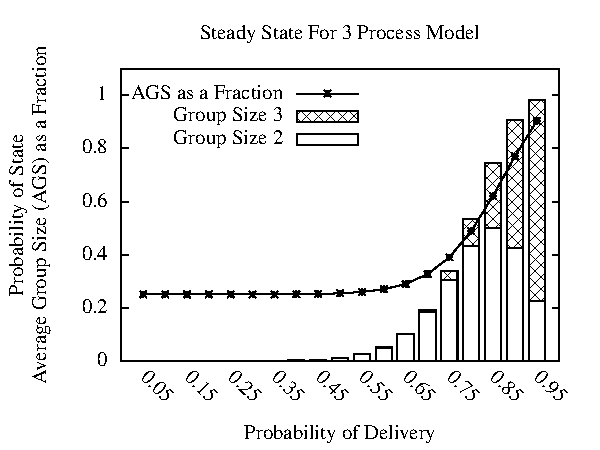
\includegraphics[width=0.6\linewidth]{ss-3process.pdf}
    \caption{Steady state distribution for 3 processes as well as the \ac{AGS} as a fraction of total processes.}
    \label{fig:ss-3process}
\end{figure}

\begin{figure}
    \centering
    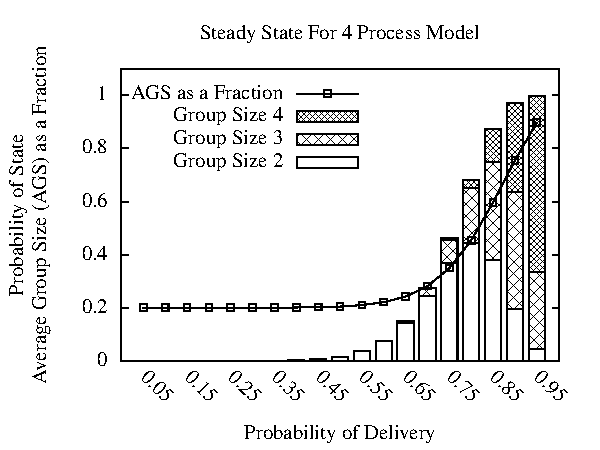
\includegraphics[width=0.6\linewidth]{ss-4process.pdf}
    \caption{Steady state distribution for 4 processes as well as the \ac{AGS} as a fraction of total processes.}
    \label{fig:ss-4process}
\end{figure}

\begin{figure}
    \centering
    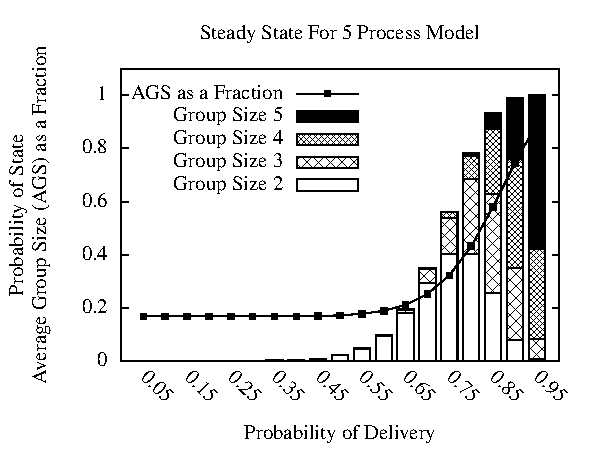
\includegraphics[width=0.6\linewidth]{ss-5process.pdf}
    \caption{Steady state distribution for 5 processes as well as the \ac{AGS} as a fraction of total processes.}
    \label{fig:ss-5process}
\end{figure}

\begin{figure}
    \centering
    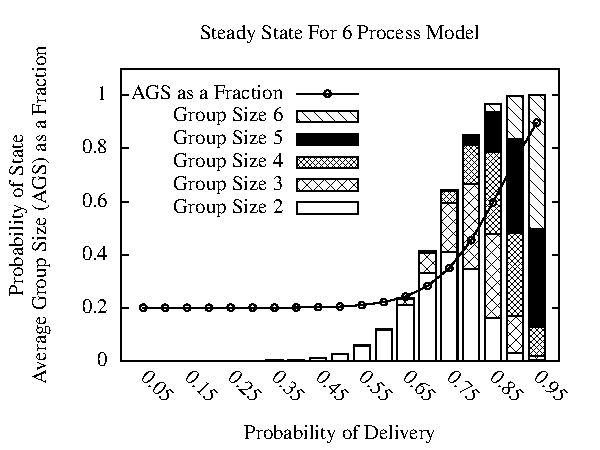
\includegraphics[width=0.6\linewidth]{ss-6process.pdf}
    \caption{Steady state distribution for 6 processes as well as the \ac{AGS} as a fraction of total processes.}
    \label{fig:ss-6process}
\end{figure}

The profile chain can be used to ensure the \ac{FREEDM} smart grid is able to continue operating despite network issues.
The profile chain can be combined with different message sending strategies to maintain service.
For example, the DGI can change to a slower mode of operation to ensure operation continues normally despite connectivity issues.
By selecting different strategies depending on the message delivery probability the DGI can offer high performance in good network conditions and an acceptable level of service during faults.
The profile chain can be extended to an arbitrary number of processes as shown in Figure \ref{fig:ss-means}.
In Figure \ref{fig:ss-means}, the steady-state of the system is used to compute a weighted average of the group size.
To compare the produced steady states, the weighted average was plotted as a percentage of all processes in the system.
Values in Figure \ref{fig:ss-means}, were plotted using Equation \ref{eq:ss-means}.
Therefore, Figure \ref{fig:ss-means}, shows the average percentage of total processes that will be in the group in a steady-state system.

\begin{figure}
    \centering
    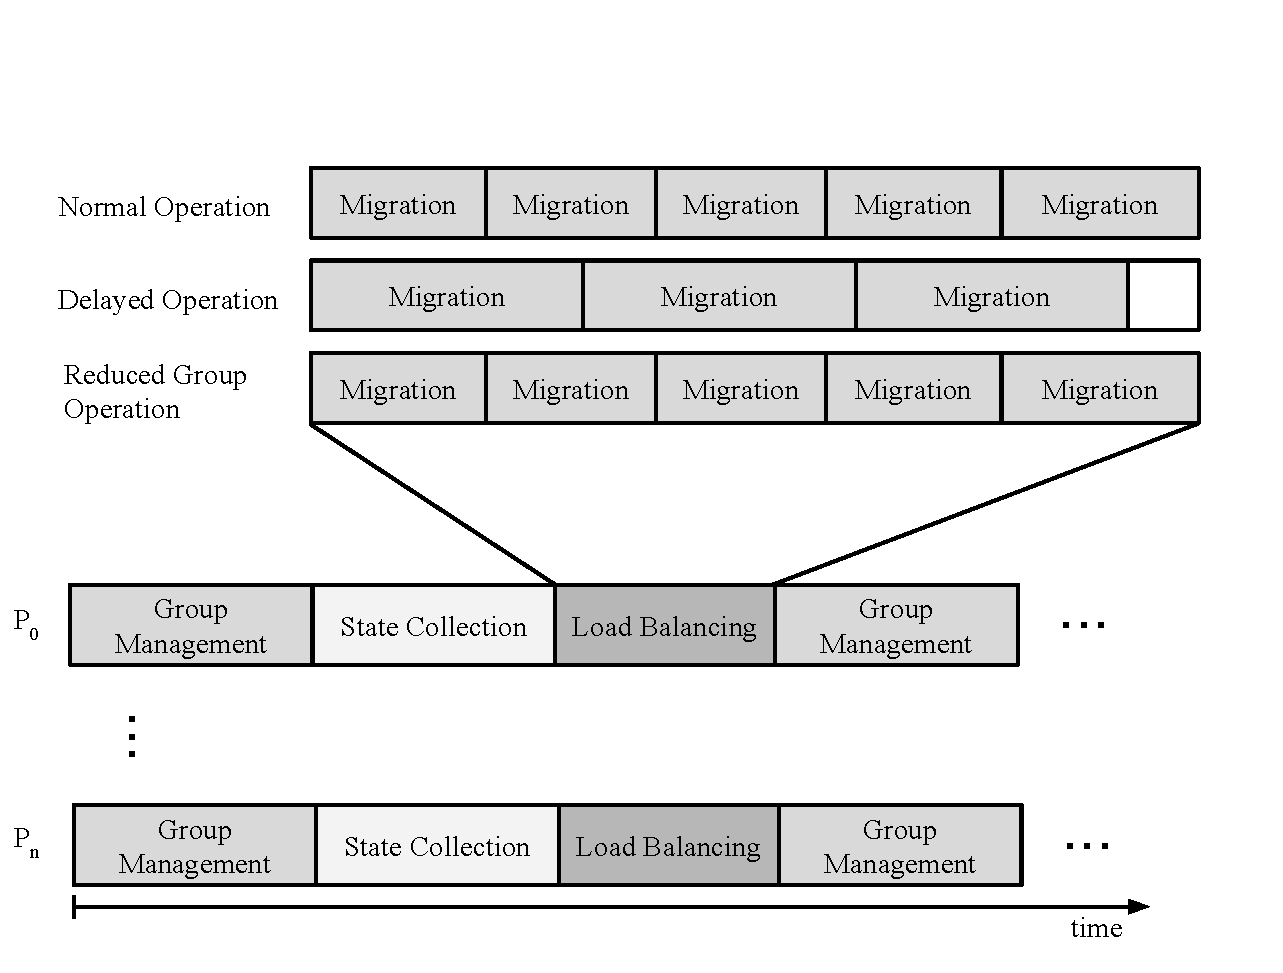
\includegraphics[width=0.75\linewidth]{schedule.pdf}
    \caption{Example DGI schedule. Normal operation accounts for a fixed number of migrations each time the load balancing module runs. Message delays reduce the number of migrations that can be completed each round. However, reducing the group size allows more migrations to be completed (because fewer messages are being exchanged) at the cost of flexibility for how those migrations are completed.}
    \label{fig:schedule}
\end{figure}

The DGI employed a round-robin schedule where each module is given a predetermined amount of time to execute.
This schedule was determined by the number of DGI that could be grouped together and the expected cyber network conditions.
Additionally, the Load Balance module, which managed the power resources was scheduled to run multiple times in a long block before the group was evaluated for failure.
This schedule is depicted in \ref{fig:schedule}.
The system began by using group management to organize groups.
Next load balancing ran to manage power resources in the created group.
Finally, state collection collected a casually consistent state to be used for reporting and offline analysis.
If message delays occurred, the number of migrations load balancing could perform was reduced.
However, by reducing the group size, the number of messages sent by load balancing could be reduced, allowing for a greater amount of work to be done.
The outcome of an election had a direct effect on how effectively the DGI can manage resources.
Therefore the steady-state analysis gives a good indication of how well the DGI could manage those resources in the future.
%Interestingly, the average group size as percentage of the total processes seems to be converging asymptotically, to a fixed value for each plotted probability as the number of processes increases.

\begin{figure}
    \centering
    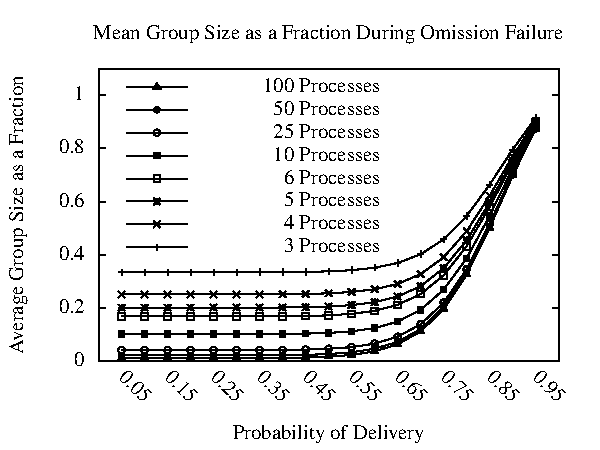
\includegraphics[width=0.6\linewidth]{ss-means.pdf}
    \caption{Average group size as a percentage of all processes in the system for larger systems.}
    \label{fig:ss-means}
\end{figure}

This information can also be used to anticipate faults and mitigate them before they occur.
Modern routers can supply an expected congestion notification as part of the IP header\cite{ECN2}.
When congestion is anticipated, the coordinator can preemptively split the group to reduce congestion.
This is possible because the algorithm's message complexity is $O(n^2)$.
Future work will combine this analysis with \ac{ECN} techniques to preemptively change the behavior of DGI to ensure a good level of service.
If dropped messages account for an omission rate of even 0.15 from future congestion, performing a coordinated group division can potentially save several rounds of transient states.
Breaking the large groups into smaller sets can drastically reduce the number of messages transmitted and help relieve congestion.
Additionally, the coordinator can design the split to ensure work can continue when the groups are split, by mixing supply and demand processes.
The division can also account for the placement of congested routers for targeted congestion relief.
Furthermore, since the required execution time is a function of group size, the DGI can use the additional execution time within the same real time schedule to use more reliable techniques to deliver messages.


In Figure \ref{fig:schedule}, Group Management's execution is broken into four steps: check, merge, ready, and cleanup.
Between each step, the DGI waits while messages and their replies are delivered.
The leader election algorithm expects that all replies arrive before the next step of the algorithm is executed.
If a message does not arrive during the wait period, before the next step of execution the message is considered lost.
If it arrives later, it is ignored by the algorithm.
While dynamically adjusting the synchronized schedule is not feasible during failure, adjusting the number of messages sent (by sending fewer "Are You Coordinator" messages, for example) is.
By sending fewer messages, the number of packets in the communication network is reduced, and the savings in processing can allow multiple delivery attempts in the scheduled wait time.
